\section{Interface}
\label{sect:kegg_interface}

\begin{figure}
    \center{
        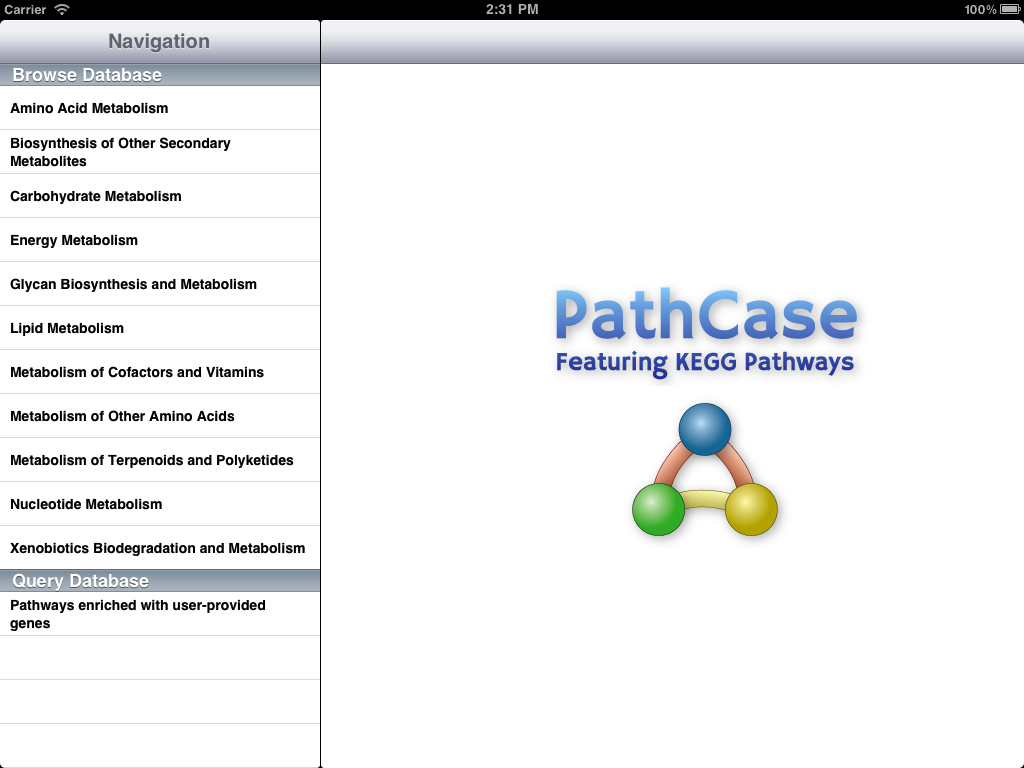
\includegraphics[width=\columnwidth]{kegg/figures/screenshot_list}}
    \caption{\label{fig:kegg_screenshot_list} List of pathways on the main screen
    of PathCase KEGG for iPad}
\end{figure}

The home screen of the KEGG app displays a list of pathways that the user can
choose from to view a graph. This screen is shown in figure
\ref{fig:kegg_screenshot_list}.

After selecting a pathway, the user enters the graph view, where they can pan
and zoom across a pathway. The view for glycolysis/gluconeogenesis is shown in
figure \ref{fig:kegg_screenshot_pathway}.

\begin{figure}[hbt]
    \center{
        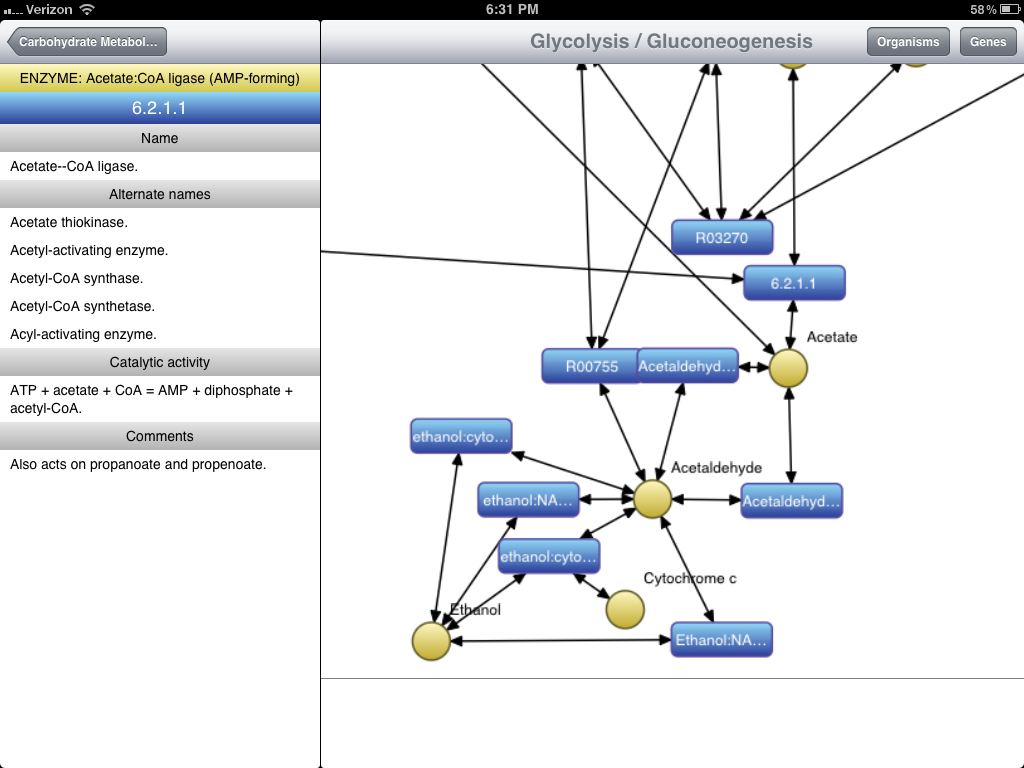
\includegraphics[width=\columnwidth]{kegg/figures/screenshot_glycolysis_gluconeogenesis}}
    \caption{\label{fig:kegg_screenshot_pathway} Scrolling,
    zooming view of Glycolysis/Gluconeogenesis}
\end{figure}

One significant difference between the MAW and KEGG apps is that the KEGG app
displays data from the ENZYME enzyme nomenclature database where possible.  The
database's data comes from the recommendations of the Nomenclature Committee of
the International Union of Biochemistry and Molecular Biology (IUBMB)
\cite{enzyme-database}. This data is shown in the sidebar of figure
\ref{fig:kegg_screenshot_pathway}, including alternate names, catalytic
activity, cofactors, and more.
